
\chapter{Aufgabe D7}
Die folgenden Graphiken zeigen die Umsetzung der Simulink-Simulation in ASCET. 
\begin{figure}[h!]
	\centering
	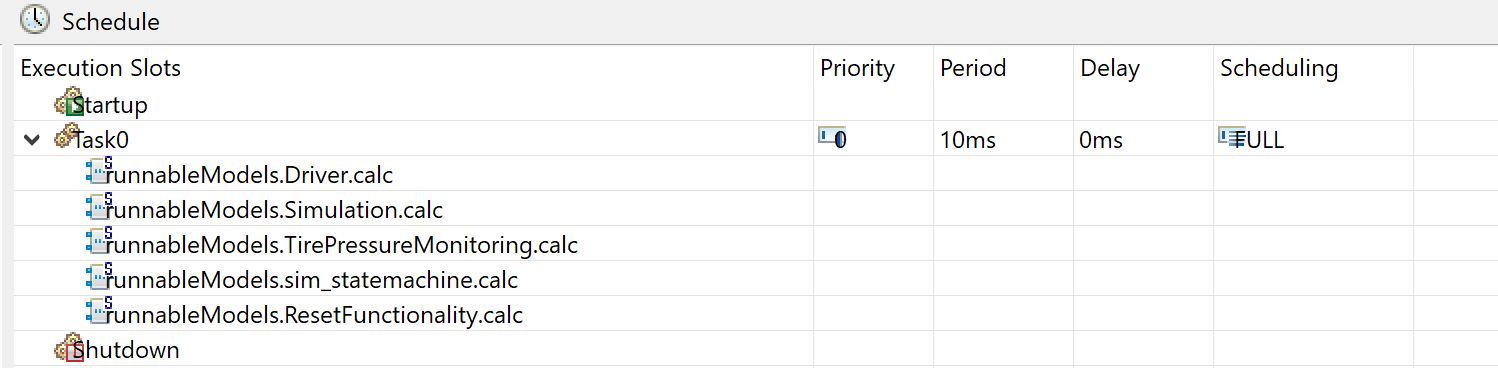
\includegraphics[width=1\linewidth]{../Graphiken/Schedule}
	\caption{ASCET Schedule}
	\label{fig:Schedule}
\end{figure}
Die Simulink-Simulation ist in ASCET in drei Teile geteilt:
\begin{itemize}
	\item Driver
	\item Simulation
	\item TirePressureMonitoring
\end{itemize}
Die weiteren Teile werden in folgenden Aufgaben weiter erläutert.
\subsubsection{Driver}
Der Driver ist ein Containermodell und enthält den Randomgenrator als Submodul.
\begin{figure}[H]
	\centering
	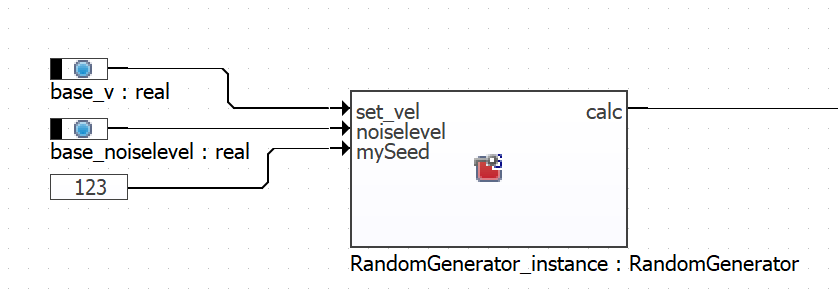
\includegraphics[width=0.7\linewidth]{../Graphiken/ASCETRandomgen.png}
	\caption{ASCET Randomgenerator}
	\label{fig:ASCETRandom}
\end{figure}
Dieser ist für jedes Rad einmal vorhanden. Eine Message sendet das jeweilige SIgnal weiter an andere Module.\\
Die Implementierung unterscheidet sich kaum von Simulink. Eine setSeed Funktionalität wurde ergänzt.
\begin{figure}[H]
	\centering
	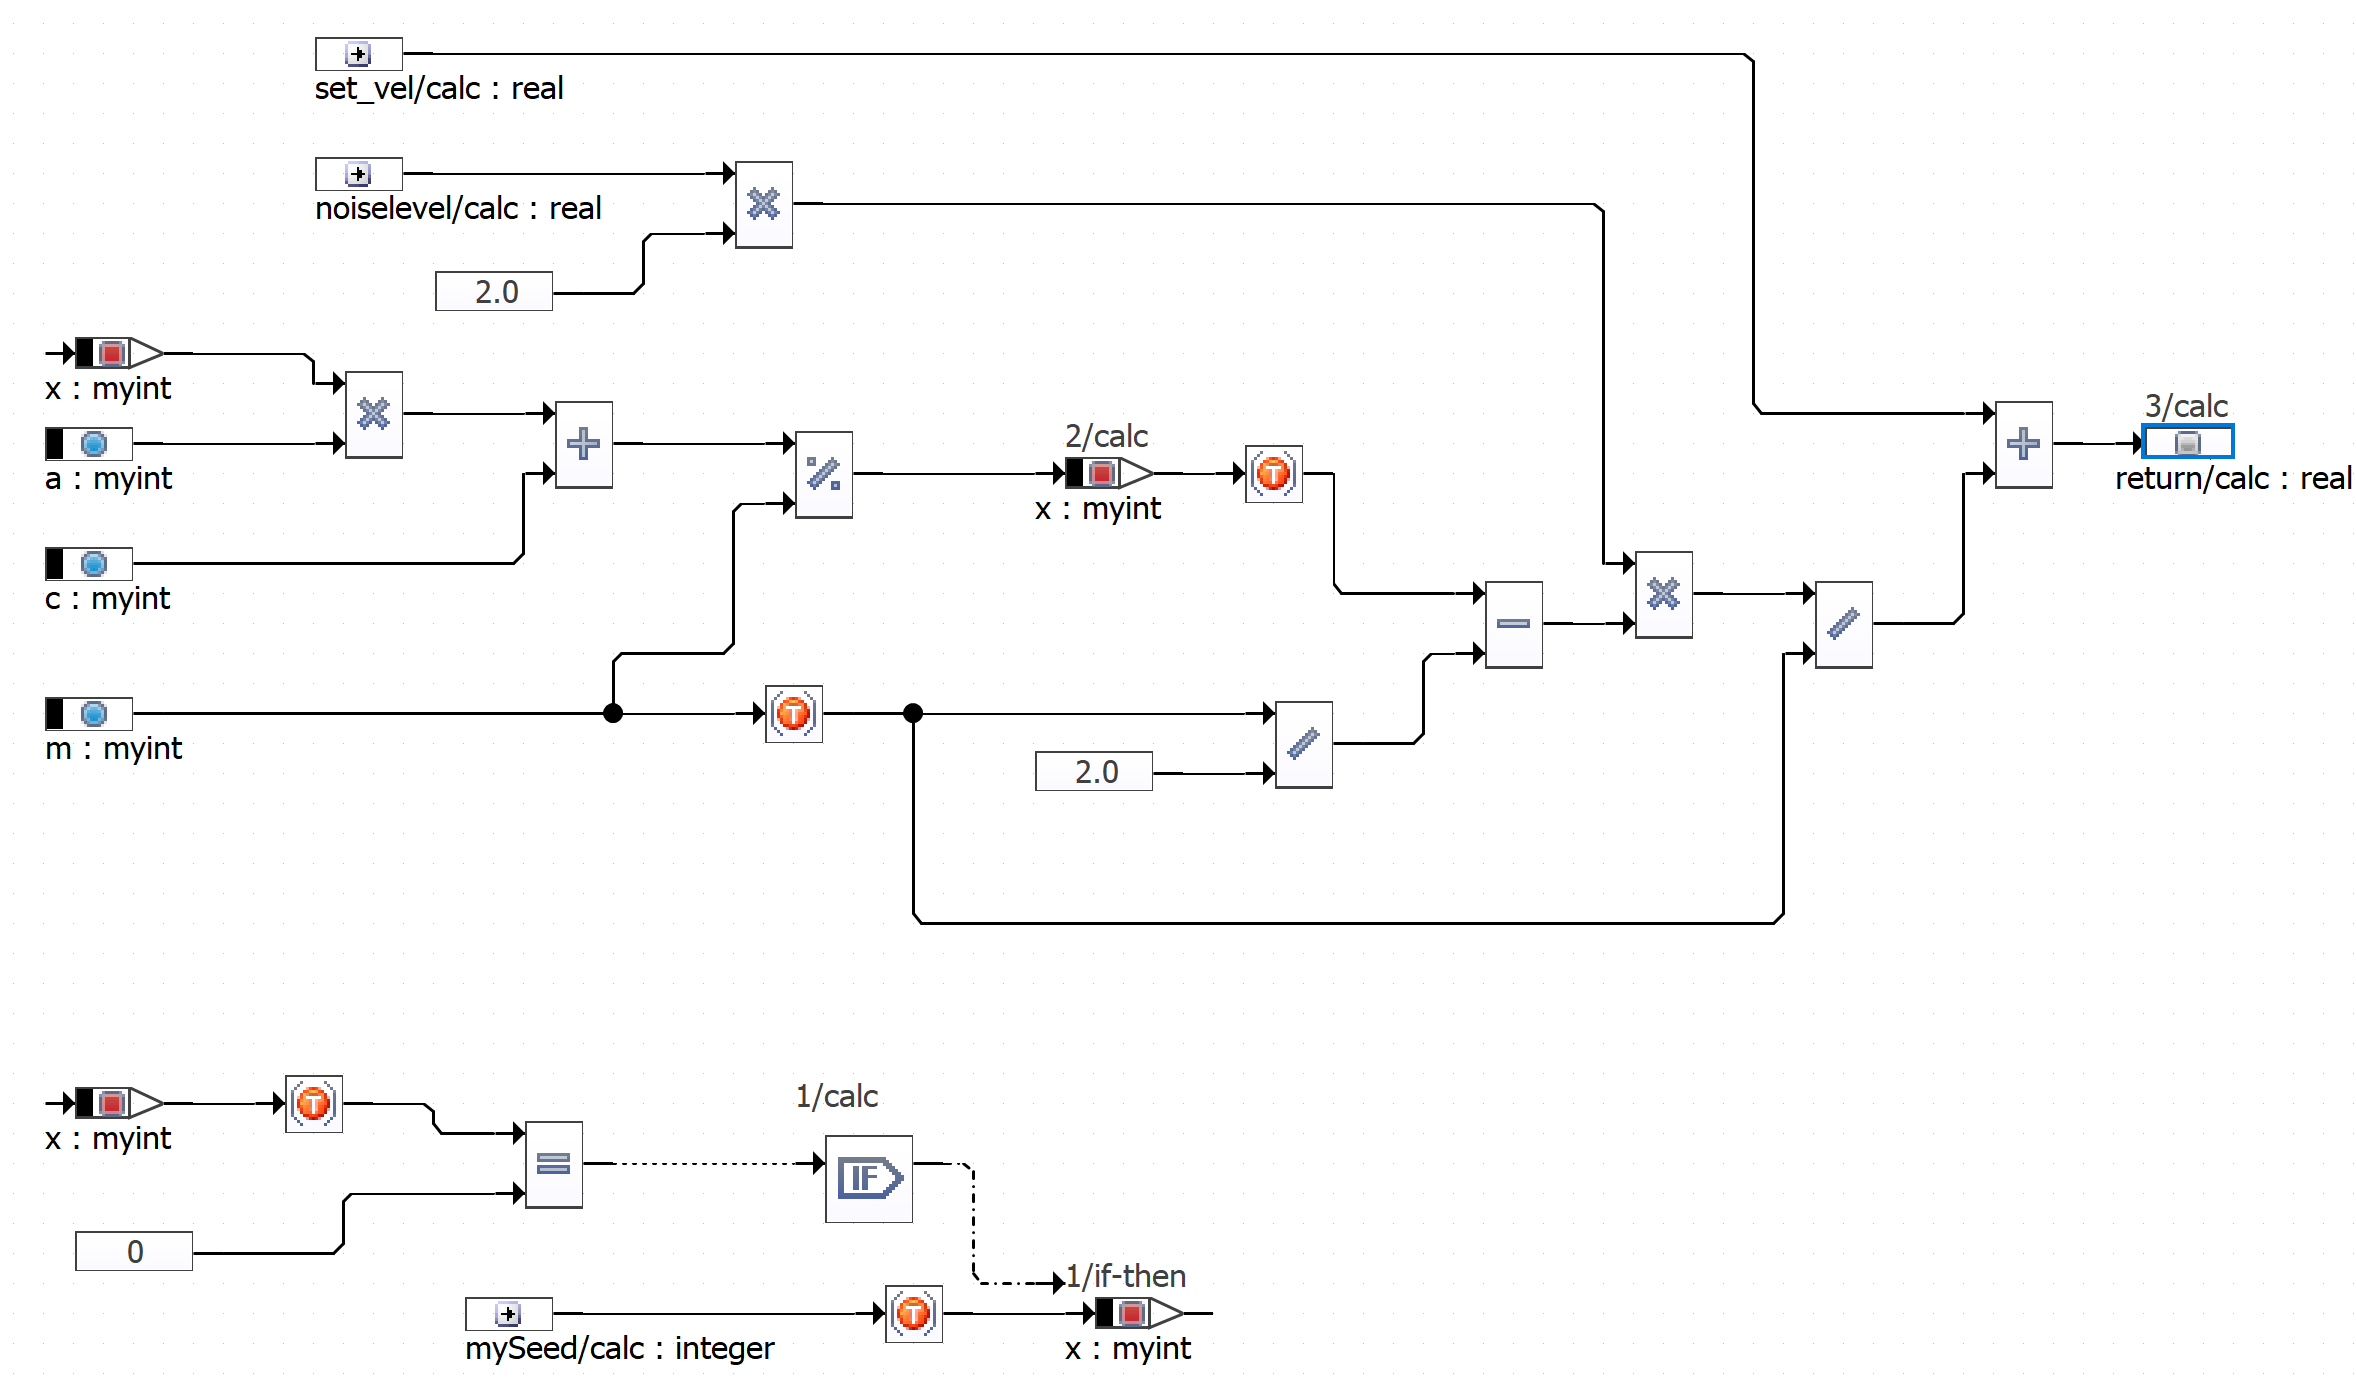
\includegraphics[width=1\linewidth]{../Graphiken/RandomGenerator.png}
	\caption{Random Number Generator}
	\label{fig:RandomGenerator}
\end{figure}
Es wird auch ein eigener Typ für die Modulooperation benötigt.
\begin{lstlisting}
type myint is integer 0 .. 1024;
\end{lstlisting}
Die Parameter sind gleich implementiert. Bei der Codegenerierung mit m = $2^{31}$ ist ein Fehler aufgetreten. Die Vermutung ist, dass dieser Wert zu groß ist. Deshalb wurde m auf $2^{10}$ gesetzt.
\begin{lstlisting}
class RandomGenerator {
characteristic myint a = 89;
characteristic myint m = 1024;
characteristic myint c = 251;
myint seed;
myint x = 0;
@generated("blockdiagram")
public real calc(real in set_vel, real in noiselevel, integer in mySeed) {
...
}
}
\end{lstlisting}

\subsubsection{Simulation}
Die Simulation berechnet, die Distanzen und Deltas in einem Submodul und schickt diese dann per Message weiter.
\begin{figure}[H]
	\centering
\includegraphics[width=1\linewidth]{../Graphiken/ModelSim}
\caption{Simulation}
\label{fig:Sim}
\end{figure}
Im Submodul wird die Strecke durch Integration mit dem dT-Element für alle vier Räder berechnet.
\begin{figure}[H]
	\centering
	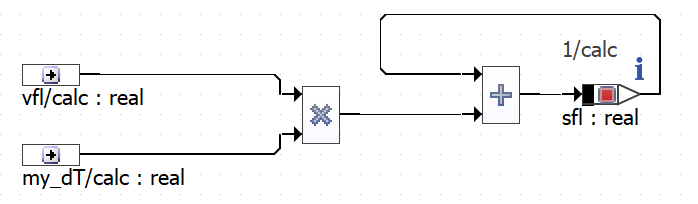
\includegraphics[width=0.6\linewidth]{../Graphiken/integrate}
	\caption{Streckenberechnung für Vornelinks}
	\label{fig:Sim}
\end{figure}
Um das 10 Sekundendelta zu erhalten wird der gespeicherte Wert von vor 10 Sekunden abgezogen (auch für alle vier Reifen).
\begin{figure}[H]
	\centering
	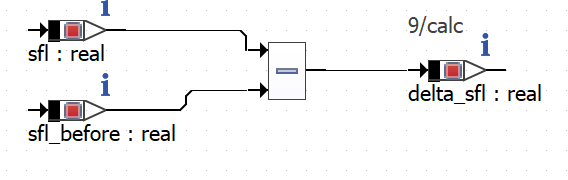
\includegraphics[width=0.5\linewidth]{../Graphiken/delta}
	\caption{Deltaberechnung}
	\label{fig:delta}
\end{figure}
Das Speichern vergangener Werte wird durch einen Buffer umgesetzt. Jeder Reifen besitzt einen eigenen Buffer.
\begin{figure}[H]
	\centering
	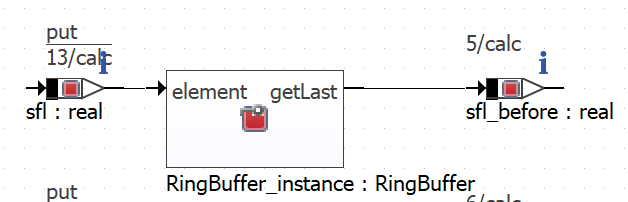
\includegraphics[width=0.6\linewidth]{../Graphiken/RinbufferApp}
	\caption{Buffer}
	\label{fig:Buffer}
\end{figure}
Der Buffer wird als Code implementiert.
\begin{lstlisting}
package components;
type s_array is array [] of real;

class RingBuffer{

	s_array buffer[1000];    
	real c;
	real swap;
	
	public void put(real element){
		swap = element;
		for(i in 0 .. 999){
		c = buffer[i];
		buffer[i] = swap;
		swap = c;
		}
	}
	
	public real getLast(){
		return buffer[999];
	}
	
	public real getIndex(integer i){
		return buffer[i];
	}
}
\end{lstlisting}
Die Codenotation ist einfacher zu implementieren und für diesen Fall auch übersichtlicher.
Um die berechneten Größen im Topmodul zugänglich zu machen, werden für die Strecken und Deltas getter-Funktionen im Code implementiert.

\subsubsection{TirePressureMonitoring}
Im Topmodul wird zum einen der Mittelwert,
\begin{figure}[H]
	\centering
	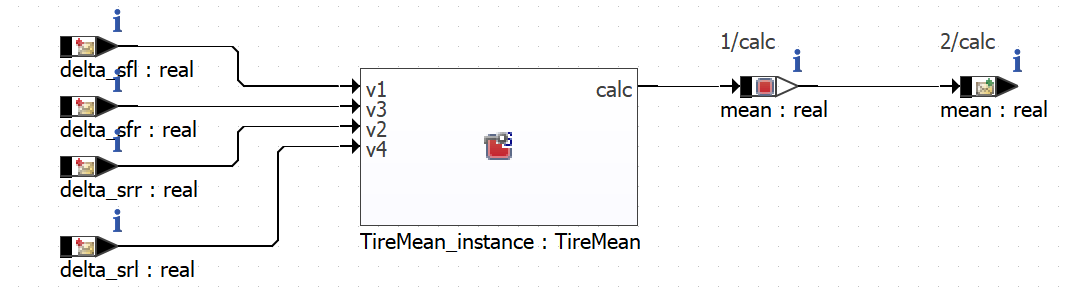
\includegraphics[width=0.7\linewidth]{../Graphiken/mean}
	\caption{Berechnung des Mittelwerts}
	\label{fig:Simittelm}
\end{figure}
und die Prozentuale Abweichung für alle Räder berechnet.
\begin{figure}[H]
	\centering
	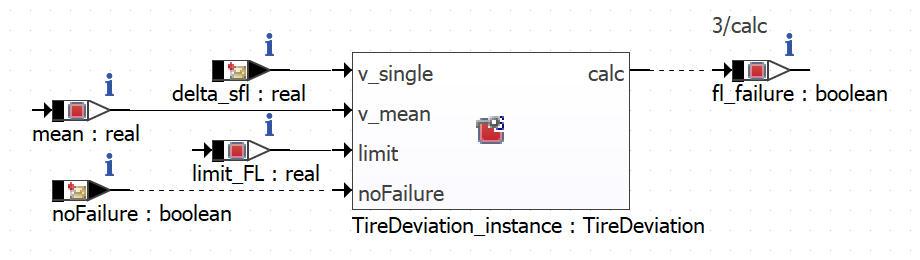
\includegraphics[width=0.7\linewidth]{../Graphiken/deviation}
	\caption{Druckabweichungsberechnung für Vornelinks}
	\label{fig:abweichung}
\end{figure}
Abschließend werden die Ergebnisse aller vier Reifen verodert.
\begin{figure}[H]
	\centering
	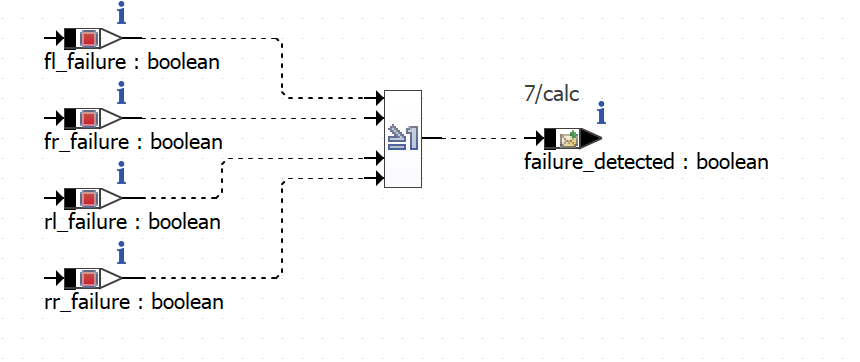
\includegraphics[width=0.7\linewidth]{../Graphiken/or}
	\caption{Streckenberechnung für Vornelinks}
	\label{fig:Sim}
\end{figure}
Die Mittelwertberechnung unterscheidet sich gar nicht vom Simulinkmodel und ist wie in \autoref{mittel} in einem Submodul wie folgt umgesetzt.
Die \autoref{fig:Model} berechnet die Strecken der einzelnen Räder. Dafür wird ein RingBuffer mit Werten befüllt. Dieser wurde mit folgendem Code umgesetzt.
\begin{figure}[H]
	\centering
	\includegraphics[width=0.8\linewidth]{../Graphiken/meanCalc}
	\caption{Mittelwertberechnung}
	\label{fig:Sim}
\end{figure}
Die Abweichungsberechnung unterscheidet sich ebenfalls nicht vom SImulink Modell und ist ebenfalls wie in \autoref{abweichung} in einem Submodul wie folgt umgesetzt.
\begin{figure}[H]
	\centering
	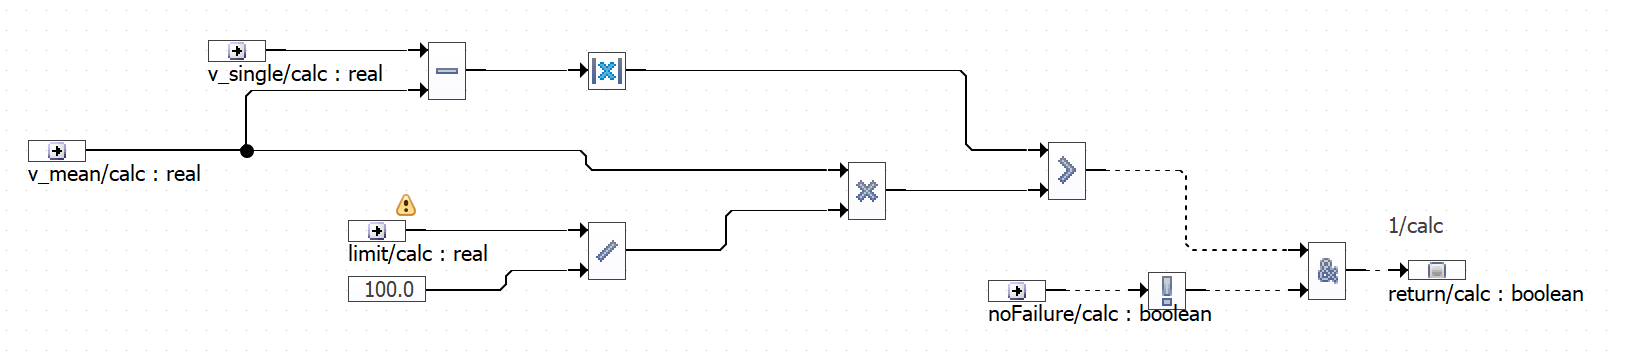
\includegraphics[width=\linewidth]{../Graphiken/devCalc}
	\caption{Mittelwertberechnung}
	\label{fig:Sim}
\end{figure}






